\documentclass[11pt,tikz,svgcolornames]{standalone}

\usepackage{fontspec}
\usepackage{unicode-math}

\setmainfont{TeX Gyre Pagella}
\setsansfont{Linux Biolinum O}
\setmathfont{TeX Gyre Schola Math}

\usepackage{ifthen}
\usepackage{amsmath}

\usepackage[d]{esvect}
\usetikzlibrary{shapes.misc}
\usetikzlibrary{arrows,arrows.meta}
\usetikzlibrary{calc,intersections, patterns, math}

\definecolor{pfeil}{RGB}{168,167,167}
\definecolor{salmon}{RGB}{250,128,114}
\definecolor{petrol}{RGB}{0, 118, 136}
\definecolor{darkgoldenrod}{RGB}{184, 134, 11}
\colorlet{petrol-lighter}{petrol!40}
\colorlet{darkgoldenrod-lighter}{darkgoldenrod!40}

\tikzset{>={Stealth[scale=1.25]}}

\begin{document}

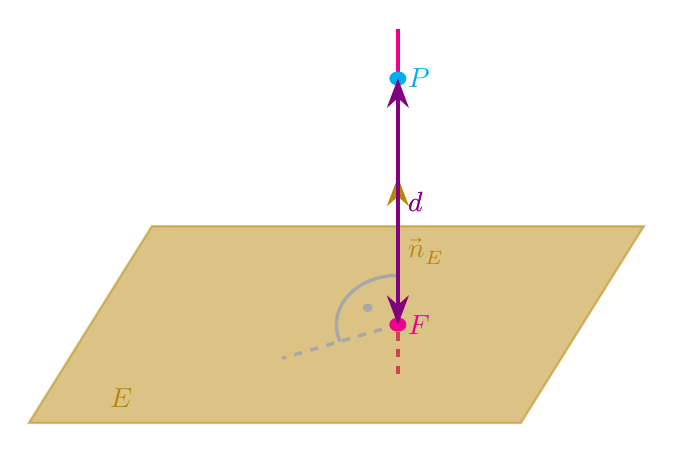
\begin{tikzpicture}[pfeil, very thick, scale=1.25,xscale=1.25]
			
	\draw[magenta,dashed] (3,0.5) -- (3,1);

	\draw[draw=darkgoldenrod, fill=darkgoldenrod, thick, opacity=0.5] (0,0) -- (4,0) -- (5,2) -- (1,2) -- cycle;
	\node[darkgoldenrod] at (0.75,0.25) {$E$};	
	\draw[dashed] (3,1) -- ++(200:1);
	\draw (3,1.5) arc(90:200:0.5);
	\draw[fill] (3,1)++(145:0.3) circle (0.025);
	\draw[darkgoldenrod,->] (3,1) -- node[right]{$\vec n_E$} (3,2.5);

	\draw[magenta] (3,1) -- (3,4);

	\draw[very thick, violet] (3,1) -- node[right] {$d$} (3,3.5);

	\draw[magenta, fill] (3,1) circle(0.055) node[right]{$F$};
	
	\draw[cyan, fill] (3,3.5) circle(0.055) node[right]{$P$};

	\draw[very thick, violet,<->] (3,1) -- node[right] {$d$} (3,3.5);

\end{tikzpicture}			

\end{document}
